\chapter{Principe de l'auralisation}

Le but de cette section est de mettre en lumière le procédé mathématique permettant l'auralisation d'une salle. Pour cela nous allons nous interesser a plusieurs notions qui rentre en jeu dans l'auralisation.

\section{Produit de convolution} % {{{1

Nous allons nous intéresser dans ce projet uniquement à des salles en taille réelle avec une source et un récepteur fixes. Dans ce cas particulier, la salle à étudier peut être assimilée à un filtre linéaire invariant par translation dans le temps. 
Pour qu'un système puisse être considéré comme linéaire, il suffit que pour des entrées $x_1(t)$ et $x_2(t)$ et leurs sorties respectives $y_1(t)$ et $y_2(t)$ on ait :
    
\begin{equation}
    \alpha x_1(t) + \gamma x_2(t) \Leftrightarrow \alpha y_1(t) + \gamma y_2(t)
\end{equation}

Dans notre cas, si 2 sons d'enveloppes et d'amplitude différentes sont émis dans une salle, il parait logique ques ces sons n'interagiront pas entre eux et que par conséquent cette équation soit vérifiée dans le cas de l'émission d'un son dans une salle avec un émetteur et recépteur fixes.
On peut dire qu'un système est invariant par translation dans le temps si, alors qu'à un temps $t$ une entrée $x(t)$ est reliée à une sortie $y(t)$ on a pour un temps $t+\tau$ une entrée $x(t+\tau)$ liée à une sortie $y(t+\tau)$ (voir figure~\ref{systeme_invariant}).

\begin{figure}[h!]
    \centering{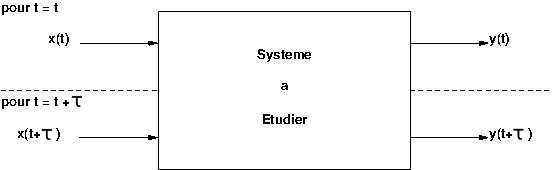
\includegraphics[width=10]{systeme_invariant.png}}
    \caption{\label{systeme_invariant} Le système à étudier est considéré invariant par translation dans le temps si on peut lier les entrées aux sorties par une fonction de transfert immuable pendant le temps considéré.}
\end{figure}

Dans le cadre de ce rapport, à la condition que ni l'émetteur ni le récepteur ne change de position et que les conditions extérieures ne fluctuent pas trop (température, pression ambiante), la réponse d'une salle à un son donné n'a \textit{a priori} aucune raison de varier dans le temps.
Une salle peut donc bien être approximée à un système linéaire
On a donc le système présenté figure~\ref{systeme_lineaire_invariant}.

%%%%%% TODO %%%%%%%
% A complèter, à décommenter.
% Retirer ensuite les banières en commentaire

% \begin{figure}[h!]
% \begin{center}
% \includegraphics[width=10cm]{ NOM DE FICHIER}
% \end{center}
% \caption{\label{systeme_lineaire_invariant} LEGENDE }
% \end{figure}

%%%%%% END TODO %%%%%%%


Comme les systèmes qui seront étudiés sont tous linéaires, on peut d'ores et déjà rappeler certaines des propriétés de ces systèmes qui seront utiles par la suite.  
Sachant que le système est linéaire, on a donc :
\begin{equation}
    \alpha x_1(t) + \gamma x_2(t) \Leftrightarrow \alpha y_1(t) + \gamma y_2(t)       
\end{equation}

Et

\begin{equation}     
    x_1(t)  \Leftrightarrow y_1(t)                 
    x_1(t -\tau) \Leftrightarrow y_1(t -\tau)                
\end{equation}

En combinant ces 2 propriétés on peut en déduire que :

\begin{equation}       
    \alpha x_1(t - \tau) + \gamma x_2(t - \tau) \Leftrightarrow \alpha y_1(t - \tau) + \gamma y_2(t - \tau)       
\end{equation}

On considère maintenant un signal quelconque $e(t)$, on peut approximer ce signal par une somme de signaux impulsionnels $a(t)$ d'amplitudes différentes et décalés dans le temps.
On a donc :

\begin{equation}        
    e(t) = \sum_{i} A_i a(t - \tau_i)
\end{equation}

Comme le système est linéaire on peut donc en déduire que la sortie du système s'écrira :

\begin{equation}        
    s(t) = \sum_{i} A_i h(t - \tau_i)
\end{equation}

Si on passe cette écriture à la limite continue, on obtient :

\begin{equation}        
    e(t) \to s(t) = \int e(\tau)h(t -\tau)d\tau
\end{equation}

Cette dernière relation est fondamentale et est nommée produit de convolution. Ce produit est dénoté par le signe $\ast$.
De plus on constate que la fonction $h(t)$ correspond à la sortie du système pour une unique impulsion envoyée en entrée (visible dans le cas ou on prend un i unique).
Cette fonction est essentielle dans le processus d'auralisation, il s'agit de la fonction de tranfert caractérisant le système dans le domaine temporelle, aussi nommée réponse impulsionnelle du système (RI).


\section{Mise en relation avec la transformée de Fourier} % {{{1


En termes de ressources et de temps de calcul, le produit de convolution est extrêmement lourd ; il est, de plus, peu maniable.
Il est toutefois possible de se servir d'une autre opération mathématique afin de rendre plus simple l'utilisation du produit de convolution.
La transformée de Fourier et l'espace de Fourier proposent des propriétés interessantes. Des algorithmes bien connus permettent de plus d'alléger le calcul et de l'accélérer (\textit{Fast Fourier Transform} notamment).
La transformée de Fourier est définie de la manière suivante:

\begin{equation}
    \mathcal{F}\{x(t)\} = \int_{-\infty}^{+\infty} x(t) e^{-2i\pi Ft} \mathrm dx
\end{equation}

Une des propriétés intéressante concerne la transformée de Fourier d'un produit de convolution :

\begin{eqnarray*}
    \mathcal{F}\left\{x(t) \ast y(t)\right\} & = & \int_{-\infty}^{+\infty} \left[x(t) \ast y(t)\right] e^{-2i\pi Ft} \mathrm dt \\
    & = & \int_{-\infty}^{+\infty} \int_{-\infty}^{+\infty} x(u)y(t - \tau ) \mathrm du e^{-2i\pi Ft} \mathrm dt \\
    & = & \int_{-\infty}^{+\infty}  \left[ \int_{-\infty}^{+\infty} x(u)y(t - \tau )  e^{-2i\pi Ft} \right] \mathrm du \mathrm dt \\
\end{eqnarray*}

On pose $v= t- u$, on a donc $t= u+v$ à $u$ fixé,

\begin{eqnarray*}
    \mathcal{F}\left\{x(t) \ast y(t)\right\} & = & \int_{-\infty}^{+\infty}  \left[ \int_{-\infty}^{+\infty} x(u)y(v)  e^{-2i\pi F(v+u)} \right] \mathrm du \mathrm dv\\
    & = & \int_{-\infty}^{+\infty}  x(u) e^{-2i\pi Fu}  \mathrm du
    \int_{-\infty}^{+\infty} y(v) e^{-2i\pi Fv} \mathrm dv \\
    & = & \mathcal{F}\left\{x(t)\right\}\cdot\mathcal{F}\left\{y(t)\right\} \\
\end{eqnarray*}

La transformée de Fourier du produit de convolution de 2 signaux est donc égale à la multiplication des transformées de Fourier de chacun des signaux.
Par conséquent, les calculs de produits de convolutions sont fait en passant par le domaine de Fourier pour l'accélération (voir le paragraphe~\ref{acceleration_des_calculs})


\section{Application à l'auralisation} % {{{1

Dans le cas d'un système linéaire on a :

\begin{equation}
e(t) \ast h(t) = s(t)
\end{equation}

Avec $e(t)$ le signal en entrée du système, $h(t)$ sa RI et $s(t)$ le signal en sortie du système pour $e(t)$ en entrée.
Dans le cas de l'auralisation d'une salle, le signal d'entrée correspond au signal anéchoïque que à émettre dans la salle et le signal de sortie au signal enregistré une fois le système excité.
Lorsque la réponse impulsionnelle est connue (celle-ci étant facilement mesurable), il est possible, à partir de celle-ci et d'un son anéchoïque, d'en déduire le son tel qu'il pourrait être perçu si le signal anéchoïque avait été réellement émis dans la salle. C'est cette opération qu'on nomme auralisation.
Il faut cependant prendre en compte d'autres phénomènes dans le procédé d'auralisation, qui seront dûs au fait que notre source impulsionnelle excitatrice et la chaîne de mesure ne sooient pas parfaites.
C'est lors de l'application des compensation pour les sources et chaînes de mesure que passer dans le domaine de Fourier sera réellement utile pour limiter la complexité des calculs de convolution par simple multiplication et soustraction de spectres.
